% !TeX root = ../main.tex
% Add the above to each chapter to make compiling the PDF easier in some editors.

\chapter{Background}\label{chapter:background}

\section{Foundations of Tensor Networks}

\subsection{Tensors}

For our discussion, it is important to define what tensors are, how they are contracted, and how they are represented in networks. A tensor is a multidimensional array that generalizes the concept of vectors and matrices to arbitrary dimensions. Formally, a tensor of order $n$ ($n$-mode tensor or rank $n$ tensor) is a collection of entries indexed by $n$ indices, each ranging over a finite set of dimension sizes. For instance, a matrix is a second-order ($n = 2$) tensor with two indices, while a vector is a first-order ($n = 1$) tensor with a single index (see Figure~\ref{fig:tensor_definition}). Tensors are fundamental objects in linear algebra and multilinear computations, enabling compact representations of high-dimensional data and operations on them. The elements of a tensor $\mathcal{T}$ are accessed via multi-indices, denoted $\mathcal{T}_{i_1, i_2, \ldots, i_n}$, where each $i_k$ ranges from 1 to $d_k$, the size of dimension $k$. The shape of a tensor, given by the tuple $(d_1, d_2, \ldots, d_n)$, determines the total number of entries, which scales as the product of all dimension sizes. This exponential growth in storage and computation with dimension and order motivates the use of structured factorizations and tensor networks, which exploit sparsity and algebraic structure to make high-dimensional problems computationally tractable.

\begin{figure}[ht]
    \centering
    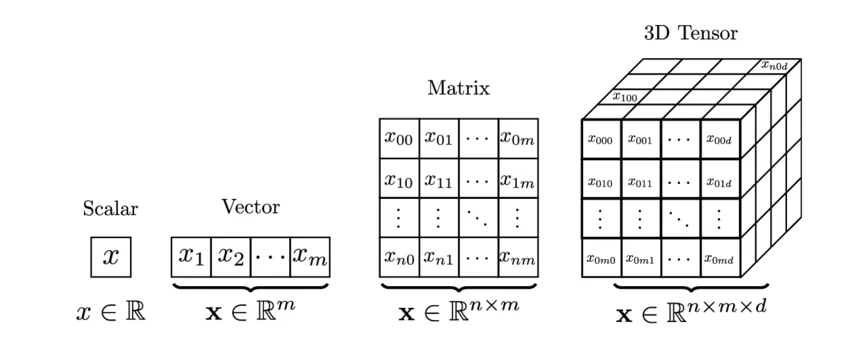
\includegraphics[width=1.0\textwidth]{figures/tensor_definition.png}
    \caption{Examples of rank-0, 1, 2, 3 tensors (i.e.\ a scalar, vector, matrix, order-3 tensor)}\label{fig:tensor_definition}
\end{figure}

\subsection{Tensor Contractions}
Tensor contractions have emerged as one of the fundamental operations on tensors. At its core, a tensor contraction represents a generalized summation over shared indices between tensors. This operation constitutes many familiar linear algebra operations such as matrix multiplication, but extends naturally to higher-order interactions. Formally, a tensor contraction between two tensors $\mathcal{A}$ and $\mathcal{B}$ over a set of shared indices $S$ is defined as:

\begin{equation}
\mathcal{C}_{j_1, \ldots, j_m, k_1, \ldots, k_n} = \sum_{i_1=1}^{d_1} \sum_{i_2=1}^{d_2} \cdots \sum_{i_r=1}^{d_r} \mathcal{A}_{i_1, \ldots, i_r, j_1, \ldots, j_m} \cdot \mathcal{B}_{i_1, \ldots, i_r, k_1, \ldots, k_n}
\end{equation}

where indices $i_1, \ldots, i_r$ are the contracted (summed) indices shared between $\mathcal{A}$ and $\mathcal{B}$, and indices $j_1, \ldots, j_m$ and $k_1, \ldots, k_n$ are the free indices that remain in the result.

A more compact and standard representation of tensor contractions is given by Einstein notation (Einstein summation convention), where repeated indices are implicitly summed over. For instance, the contraction above can be written concisely as:

\begin{equation}
\mathcal{C}_{jk} = \mathcal{A}_{ij} \mathcal{B}_{ik}
\end{equation}

where $i$ is the repeated (contracted) index and is implicitly summed over all its dimensions, while $j$ and $k$ are free indices appearing in the result. This notation extends naturally to higher-order tensors and multiple contractions, making it a powerful tool for expressing complex tensor network computations in a compact form.

\begin{figure}[ht]
    \centering
    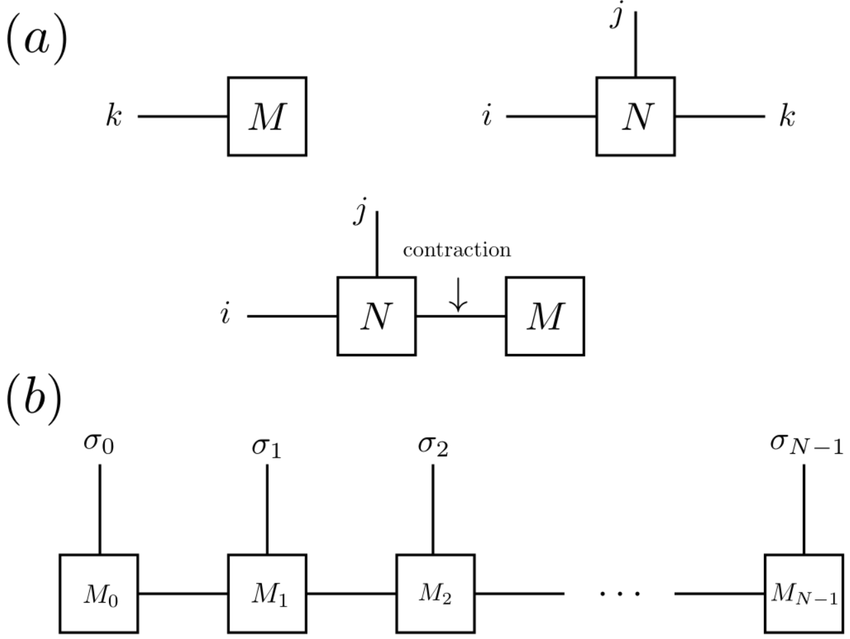
\includegraphics[width=1.0\textwidth]{figures/tensor_network_representation.png}
    \caption{(a), on the top, displays a vector, $M$, and a rank-3 tensor, $N$, contracted across their common leg $k$; (b), on the bottom, displays a complex network of $N$ tensors chained in a tensor train, commonly known as a \ac{MPS}}\label{fig:tensor_network_representation}
\end{figure}

\subsection{Tensor Networks}

However, this is not the only way to effectively represent complex contractions of networks; we can also draw them in tensor networks. A tensor network is a graphical representation of a set of tensors and their contraction structure, where nodes represent tensors and edges represent shared indices. 

In this graphical framework, each tensor is depicted as a node (typically drawn as a circle, square, or other shape), with a number of lines (legs) extending from it equal to the tensor's order. Each leg corresponds to one index of the tensor. When two legs are connected by an edge, the corresponding indices are contracted (summed over). Free indices, which do not participate in contractions, are drawn as dangling legs extending from the network.

Consider a simple example: contracting two tensors $\mathcal{A}_{ij}$ and $\mathcal{B}_{jk}$ to produce $\mathcal{C}_{ik}$. In tensor network notation, $\mathcal{A}$ appears as a node with two legs (for indices $i$ and $j$), and $\mathcal{B}$ appears as a separate node with two legs (for indices $j$ and $k$). The leg corresponding to index $j$ in $\mathcal{A}$ is connected to the leg corresponding to index $j$ in $\mathcal{B}$, indicating that these indices are contracted. The remaining legs (corresponding to $i$ and $k$) dangle freely, representing the free indices of the result tensor $\mathcal{C}$. Figure~\ref{fig:tensor_network_representation} illustrates this concept with more examples.

More complex tensor networks can compactly represent intricate contraction patterns that would be cumbersome to express algebraically. The graphical representation immediately reveals the structure of the network i.e., which tensors share indices, the connectivity pattern, and which indices remain uncontracted. This makes tensor network diagrams important for visualizing and reasoning about large-scale contractions~\cite{biamonte2017tensor}. 

\section{Basic Linear Algebra Subprograms} 
\ac{BLAS} is a standardized specification for low-level linear algebra operations that serves as a foundation for high-performance numerical computing. Originally developed in the late 1970s~\cite{lawson1979basic}, \ac{BLAS} provides a portable and efficient interface for fundamental vector and matrix operations, enabling libraries and applications to achieve near-optimal performance across diverse hardware architectures.

\ac{BLAS} operations are organized into three hierarchical levels, each characterized by the computational intensity (ratio of arithmetic operations to memory accesses) and scope of the operations:

\subsection{Level 1: Vector Operations}
Level 1 \ac{BLAS} conserns with scalar and vector operations with computational complexity $O(n)$, where $n$ is the vector length. These operations include vector addition, scalar multiplication, dot products, and norm calculations. Due to their linear computational intensity and high memory-to-computation ratio, Level 1 operations are memory-bound and exhibit poor cache utilization. Examples include \texttt{AXPY} (scaled vector addition) (\ref{eq:axpy}), \texttt{DOT} (dot product), and \texttt{NRM2} (Euclidean norm).

\begin{equation}
    y \leftarrow \alpha x + y \quad
\label{eq:axpy}
\end{equation}

\subsection{Level 2: Matrix-Vector Operations}
Level 2 \ac{BLAS} optimizes matrix-vector operations with computational complexity $O(n^2)$, including matrix-vector products, rank-one updates, and triangular system solves. These operations have moderate computational intensity and remain memory-bound on most modern architectures. Common Level 2 operations include \texttt{GEMV} (general matrix-vector multiply) (\ref{eq:gemv}) and \texttt{GER} (general rank-one update).

\begin{equation}
    y \leftarrow \alpha A x + \beta y
\label{eq:gemv}
\end{equation}

\subsection{Level 3: Matrix-Matrix Operations}
Level 3 \ac{BLAS} covers matrix-matrix operations with computational complexity $O(n^3)$, such as matrix multiplication and triangular solves. These operations exhibit high computational intensity and can achieve efficient cache reuse through careful data blocking and tiling strategies. Level 3 operations are typically compute-bound on modern hardware, making them suitable targets for optimization and parallelization. The \ac{GEMM} (\ref{eq:gemm}) operation is the cornerstone of Level 3 \ac{BLAS}.

\begin{equation}
    C \leftarrow \alpha A B + \beta C
\label{eq:gemm}
\end{equation}


Efficient implementations of \ac{BLAS}, such as ATLAS, Open\ac{BLAS}, and Intel MKL, are critical for achieving high performance in scientific computing and machine learning applications~\cite{goto2008anatomy}. In the context of tensor contractions, \ac{BLAS} operations, particularly Level 3 \ac{GEMM}, serve as the primary computational kernel when contractions are transformed into matrix multiplications.

\section{High-performance Matrix-Matrix Multiplication Implementations}

The work presented uses the \texttt{\ac{TCCG}}~\cite{tccg2016a} library as its high-performance matrix-matrix multiplication engine. \texttt{\ac{TCCG}} is designed specifically to deliver efficient \ac{GEMM} kernels across modern CPU architectures by combining the algorithmic principles of blocked matrix multiplication with architecture-aware microkernel generation.

At the highest level, \texttt{\ac{TCCG}} decomposes the computation into a hierarchy of tiles. The input matrices are partitioned into blocks that fit into the different levels of the processor cache, which reduces main-memory traffic and improves data reuse. The blocked structure also enables the library to expose parallelism naturally: independent blocks can be computed concurrently across CPU cores, while each core operates on cache-resident panels of the matrices.

A central feature of \texttt{\ac{TCCG}} is its use of a carefully tuned microkernel. The microkernel computes a small block of the result matrix using registers and vector instructions, often with explicit loop unrolling and packing of input matrix panels. This organization minimizes the number of memory accesses per floating-point operation, which is essential for reaching high fractions of peak performance on modern processors.

The library also supports explicit matrix packing, where subblocks of the input matrices are copied into contiguous, cache-friendly buffers before the inner product is evaluated. Packing eliminates irregular memory access patterns that occur in standard row-major or column-major layouts, and it allows the microkernel to consume data in a streaming fashion. In \texttt{\ac{TCCG}}, the packed panels are chosen to align with the target architecture's cache line size and vector width.

Beyond blocking and packing, \texttt{\ac{TCCG}} implements an adaptive blocking strategy for common matrix shapes. For square matrices, the blocking factors are selected to balance between the L1 / L2 cache capacities and the cost of data movement. For rectangular matrices, the library selects block sizes to maintain high utilization of the inner microkernel while avoiding excessive padding or wasted computation.

It is important to emphasize that \texttt{\ac{TCCG}} is not just treated as a black-box library, but integrated into the overall implementation. Its performance model is based on the same principles discussed earlier in this chapter: increasing arithmetic intensity, maximizing cache reuse, and exposing parallelism through block-level decomposition. When tensor contractions are mapped to matrix-matrix multiplications, \texttt{\ac{TCCG}} provides the low-level kernel that performs these multiplications efficiently, making the overall tensor contraction implementation practical for large-scale problems.

\section{High-performance Tensor Contraction Implementations}

The main tensor transposition engine used in this work is the \ac{HPTT} library~\cite{springer2017hptt}. \ac{HPTT} addresses a data-movement-centric bottleneck that is ubiquitous in tensor-based codes. While a single \ac{GEMM} call can be made very fast, the full contraction pipeline often requires rearranging tensor data, and inefficient transpositions can dominate runtime if not handled carefully.

\ac{HPTT} implements multidimensional, out-of-place tensor transpositions using the same high-performance principles introduced earlier for matrix multiplication: blocking, explicit vectorization, a small hand-tuned micro-kernel, and parallelization. Concretely, \ac{HPTT} decomposes any higher-order permutation into a nest of loops surrounding a micro-kernel that performs a small, cache-resident element reordering. This decomposition has three practical advantages: (1) the micro-kernel can be hand-vectorized for the target instruction set (e.g., AVX, NEON), (2) blocking at multiple levels improves cache reuse and reduces off-chip bandwidth requirements, and (3) the loop nest exposes both data- and task-level parallelism for multicore execution.

\begin{figure}[ht]
    \centering
    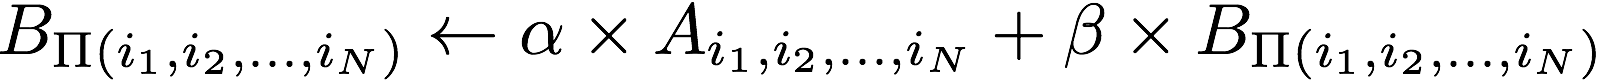
\includegraphics[width=0.8\textwidth]{figures/hptt_equation.png}
    \caption{Illustration of \ac{HPTT}'s tensor transposition semantics and permutation notation (image source: springer13/hptt).}\label{fig:hptt_equation}
\end{figure}

An important engineering feature of \ac{HPTT} is its optional autotuning framework. At plan creation time, the library can either estimate good implementation parameters from a performance model (fast) or explore a search space of loop orders, blocking factors, and parallelization strategies (measure/patient modes) to find the best-performing schedule for the current tensor shape and hardware. This behavior is analogous to FFTW's planner~\cite{frigo2005fftw} and makes \ac{HPTT} robust in applications where tensor sizes and permutations are only known at runtime.

\ac{HPTT} also supports explicit matrix/tensor packing and specializes micro-kernels to align with cache line sizes and vector register widths, thereby minimizing irregular memory accesses and enabling streaming consumption of input data. The library exposes simple C, C++, and Python interfaces for creating a transposition plan (with or without autotuning) and executing it, for example see Figure~\ref{fig:hptt_example}.

\begin{figure}[ht]
    \begin{lstlisting}[language=C++]
    #include <hptt.h>

    // allocate tensors
    float A* = ...
    float B* = ...

    // specify permutation and size
    int dim = 6;
    int perm[dim] = {5,2,0,4,1,3};
    int size[dim] = {48,28,48,28,28};

    // create a plan (shared_ptr)
    auto plan = hptt::create_plan( perm, dim, 
                                alpha, A, size, NULL, 
                                beta,  B, NULL, 
                                hptt::ESTIMATE, numThreads);

    // execute the transposition
    plan->execute();
    \end{lstlisting}  
    \caption{Example usage of \ac{HPTT}'s C++ interface from the library's documentation.}\label{fig:hptt_example}
\end{figure}

In practice, integrating \ac{HPTT} as the transposition layer in a tensor contraction pipeline significantly reduces the overall runtime, because the cost of rearranging tensor data becomes comparable, if not superior, to the cost of the high-performance \ac{GEMM} kernels if not optimized.